\documentclass[a4paper,14pt]{extarticle}

\usepackage[utf8x]{inputenc}
\usepackage[T1]{fontenc}
\usepackage[russian]{babel}
\usepackage{hyperref}
\usepackage{indentfirst}
\usepackage{here}
\usepackage{array}
\usepackage{graphicx}
\usepackage{caption}
\usepackage{subcaption}
\usepackage{chngcntr}
\usepackage{amsmath}
\usepackage{amssymb}
\usepackage[left=2cm,right=2cm,top=2cm,bottom=2cm,bindingoffset=0cm]{geometry}
\usepackage{multicol}
\usepackage{multirow}
\usepackage{titlesec}
\usepackage{listings}
\usepackage{color}
\usepackage{enumitem}
\usepackage{cmap}
\usepackage{underscore}
\usepackage{indentfirst}
\usepackage{array}
\newcolumntype{M}[1]{>{\centering\arraybackslash}m{#1}}

\definecolor{green}{rgb}{0,0.6,0}
\definecolor{gray}{rgb}{0.5,0.5,0.5}
\definecolor{purple}{rgb}{0.58,0,0.82}

\lstdefinelanguage{none}{}

\lstset{
	language={SQL},
	inputpath={../sql/},
	backgroundcolor=\color{white},
	commentstyle=\color{green},
	keywordstyle=\color{blue},
	numberstyle=\scriptsize\color{gray},
	stringstyle=\color{purple},
	basicstyle=\ttfamily\small,
	breakatwhitespace=false,
	breaklines=true,
	captionpos=b,
	keepspaces=true,
	numbers=left,
	numbersep=5pt,
	showspaces=false,
	showstringspaces=false,
	showtabs=false,
	tabsize=4,
	texcl=true,
	extendedchars=false,
	frame=single,
	morekeywords={IF, BIGSERIAL, SERIAL, TEXT, BIGINT, MONEY, BOOLEAN, REFERENCES}
}

\renewcommand{\le}{\ensuremath{\leqslant}}
\renewcommand{\leq}{\ensuremath{\leqslant}}
\renewcommand{\ge}{\ensuremath{\geqslant}}
\renewcommand{\geq}{\ensuremath{\geqslant}}
\renewcommand{\epsilon}{\ensuremath{\varepsilon}}
\renewcommand{\phi}{\ensuremath{\varphi}}
\renewcommand{\thefigure}{\arabic{figure}}
\newcommand{\code}[1]{\texttt{#1}}
\newcommand{\caret}{\^{}}

\titleformat*{\section}{\large\bfseries} 
\titleformat*{\subsection}{\normalsize\bfseries} 
\titleformat*{\subsubsection}{\normalsize\bfseries} 
\titleformat*{\paragraph}{\normalsize\bfseries} 
\titleformat*{\subparagraph}{\normalsize\bfseries} 

\counterwithin{figure}{section}
\counterwithin{equation}{section}
\counterwithin{table}{section}
\newcommand{\sign}[1][5cm]{\makebox[#1]{\hrulefill}}
\newcommand{\equipollence}{\quad\Leftrightarrow\quad}
\newcommand{\no}[1]{\overline{#1}}
\graphicspath{{../pics/}}
\captionsetup{justification=centering,margin=1cm}
\def\arraystretch{1.3}
\setlength\parindent{5ex}
\titlelabel{\thetitle.\quad}

\setitemize{topsep=0.5em, itemsep=0em}
\setenumerate{topsep=0.5em, itemsep=0em}

\begin{document}

\begin{titlepage}
\begin{center}
	Санкт-Петербургский Политехнический Университет Петра Великого\\[0.3cm]
	Институт компьютерных наук и технологий \\[0.3cm]
	Кафедра компьютерных систем и программных технологий\\[4cm]
	
	\textbf{ОТЧЕТ}\\ 
	\textbf{по лабораторной работе}\\[0.5cm]
	\textbf{<<Разработка прикладного протокола>>}\\[0.1cm]
	Технологии компьютерных систем\\[3.0cm]
\end{center}

\begin{flushright}
	\begin{minipage}{0.45\textwidth}
		\textbf{Работу выполнил студент}\\[3mm]
		группа 43501/3 \hfill Крылов И.С.\\[5mm]
		\textbf{Работу принял преподаватель}\\[5mm]
		\sign[3cm] \hfill Зозуля А.В. \\[5mm]
	\end{minipage}
\end{flushright}

\vfill

\begin{center}
	Санкт-Петербург\\[0.3cm]
	\the\year
\end{center}
\end{titlepage}

\addtocounter{page}{1}

\tableofcontents
\newpage

\section{Техническое задание}
\textbf{Система терминального доступа}
\begin{itemize}

\item \textbf{Задание}

\hspace{14pt} Разработать клиент-серверную систему терминального доступа, позволяющую клиентам подсоединяться к серверу и выполнять элементарные команды операционной системы.

\item \textbf{Основные возможности серверного приложения}
\begin{enumerate}
\item Прослушивание определенного порта
\item Обработка запросов на подключение по этому порту от клиентов
\item Поддержка одновременной работы нескольких терминальных клиентов через механизм нитей
\item Проведение аутентификации клиента на основе полученных имени пользователя и пароля

\item Выполнение команд пользователя:
\begin{itemize}
\item[>] ls – выдача содержимого каталога
\item[>] cd – смена текущего каталога
\item[>] who – выдача списка зарегистрированных пользователей с указанием их текущего каталога
\item[>] kill – Привилегированная команда. Завершение сеанса другого пользователя
\item[>] logout – выход из системы
\end{itemize}

\item Принудительное отключение клиента
\end{enumerate}

\item \textbf{Клиентское приложение должно реализовывать следующие функции:}
\begin{enumerate}
\item Установление соединения с сервером
\item Посылка аутентификационных данных клиента (имя и пароль)
\item Посылка одной из команд (ls, cd, who, kill, logout) серверу
\item Получение ответа от сервера
\item Разрыв соединения
\item Обработка ситуации отключения клиента сервером или другим клиентом
\end{enumerate}

\item \textbf{Настройки приложений} 

\hspace{14pt} Разработанное клиентское приложение должно предоставлять пользователю настройку IP-адреса или доменного имени удалённого терминального сервера и номера порта, используемого
сервером. Разработанное серверное приложение должно хранить аутентификационные данные для вех пользователей, а также списки разрешенных каждому пользователю команд.

\item \textbf{Методика тестирования} 

\hspace{14pt}  Для тестирования приложений запускаетсятерминальный сервер и несколько клиентов. В процессе тестирования проверяются основные возможности сервера по параллельной работе нескольких клиентов, имеющих различные привилегии (списки разрешенных команд). Проверяется корректность выполнения всех команда в различных ситуациях.

\end{itemize}

\section{Прикладной протокол}

Для реализации технического задания был разработан прикладной протокол передачи данных.

\subsection{Запрос}

Протоколом задаётся два формата запроса для взаимодействия клиента с сервером:

\begin{itemize}
\item запрос аутентификации с помощью пары логин:пароль \ref{tab:request_login}
\item запрос выполнения определённой команды \ref{tab:request_command} 
\end{itemize}

\begin{table}[h]
	\centering
	\begin{tabular}[center]{| M{12.5cm} | M{2.5cm} |}
	\hline
	Login:Password: & Package Index \\ \hline
	[ 0 - 507 ] & [ 508 - 511 ] \\
	\hline
	\end{tabular}
	\caption{Формат запроса аутентификации}
	\label{tab:request_login}
\end{table}

\begin{table}[h]
	\centering
	\begin{tabular}[center]{| M{2.5cm} | M{2.0cm} | M{7.0cm} | M{2.5cm} |}
	\hline
	Message Length & Command Descriptor & Command Parameters & Package Index \\ \hline
	[ 0 - 3 ] & [ 4 ] & [ 5 - 507 ] & [ 508 - 511 ] \\
	\hline
	\end{tabular}
	\caption{Формат запроса выполнения команды}
	\label{tab:request_command}
\end{table}

Оба запроса имеют одинаковый размер - 512 байт. 

\textbf{В таблице формата аутентификации \ref{tab:request_login}:}
\begin{itemize}
\item Login:Password - поле, содержащее передаваемые клиентом логин и пароль, необходимые для подключения к серверу. Протоколом задается формат ввода пары следующим образом:
\begin{table}[h]
	\centering
	\begin{tabular}{| l l l l |}
	\hline
	[login] & : & [password] & : \\ 
	\hline
	\end{tabular}
\end{table}

Поле занимает 508 байт, задавая тем самым максимально возможнуюю длинну пары логин:пароль равной 508 символам.

\item Package Index - поле, хранящее индекс пересылаемого пакета. Благодаря наличию этого поля протокол гарантирует последовательный приём пакетов (защита от перемешивания). Так же, контроль номера пакета усложняет возможность атаки с имитацией адреса клиента поторонними. Длина поля - 4 байта, что позволяет обеспечить до 9999 последовательных запросов клиента серверу. В условиях технического задания данная продолжительность взаимодействия клиента с сервером более чем достаточна. При превышении этого значения клиент будет отключён от сервера. Тем самым гарантируется пресечение чрезмерно активного трафика, исходящего от клиента, который может свидетельствовать о зловредном характере запросов клиента
\end{itemize}


\textbf{В таблице запроса выполнения команды \ref{tab:request_command}:}
\begin{itemize}
\item Message Length - длина параметров команды. В случае если команда не имеет параметров, данное поле заполняется нулями. Под данное поле выделено 4 байта.
\item Command Descriptor - целое число - дескриптор команды, однозначно определяющий требуемую команду:
\begin{itemize}
\item[-] 1 – выдача содержимого каталога ls
\item[-] 2 – смена текущего каталога cd
\item[-] 3 – выдача списка зарегистрированных пользователей с указанием их текущего каталога who
\item[-] 4 – Привилегированная команда. Завершение сеанса другого пользователя kill
\item[-] 5 – выход из системы logout
\end{itemize}
Список поддерживаемых протоколом команд ограничиваются пятью, вследствии чего под дескриптор задачи выделено поле в 1 байт. Использование схемы взаимодействия клиента с сервером посредством передачи дескприптора команды снимает с сервера задачу проверки правильности введённой с консоли пользователем команды, тем самым минимизируя количество пересылаемых пакетов и ускоряя работу сервера.

\item Command Parameters - поле длинной 499 байт, содержит параметры команд: cd и kill
\item Package Index - поле, хранящее индекс пересылаемого пакета. Идентично одноимённому полю запроса аутентификации
\end{itemize}

\subsection{Ответ}
В соответствии с имеющимися форматами запросов, протокол определено два формата ответа:
\begin{itemize}
\item ответ аутентификации
\item ответ выполнения команды
\end{itemize}

\textbf{Ответ аутентификации} - пакет длинной 1 байт, содержащий код результата аутентификации (Таблица \ref{tab:response_login}):
\begin{itemize}
\item[-] 0 - неверная пара логин:пароль, отказ в доступе
\item[-] 1 - аутентификация прошла успешно, получен доступ к удалённому терминалу
\item[-] 2 - пользователь с данным логином уже вошёл в систему с другого устройства, отказ в доступе
\item[-] * - неверный формат ввода, отказ в доступе. Имеет специальное назначение для ответа выолнения команды
\end{itemize}

\textbf{Ответ выполнения команды} - пакет длинной 8192 байт, содержащий результат выполнения команды на удалённом терминале (Таблица \ref{tab:response_command}).

Исключительной ситуацией является попытка запроса на выполнение команды клиентом, сеанс которого был завершён другим пользователем, обладающим правами администратора. Такая ситуация возможна исключительно при использовании протокола UDP, вследствие того, что отключение клиента происходит по таймауту запроса ответа от сервера. В таком случае в качестве ответа на запрос посылается однобайтовый ответ аутентификации "*", обёрнутый в формат ответа выполнения команды с помещением на первый (с индексом [0]) байт. Особенности устройства файловых систем ОС Windows и UNIX-подобных исключает возможность использования символа "*" в названиях файлов и директорий. Протоколом же запрещено создание логинов, начинающихся с символа "*". Тем самым ислючается наличие и ошибочное обнаружение символа "*" в стандартном ответе выолнения команды.

\begin{table}[h]
	\centering
	\begin{tabular}[center]{| M{4cm} |}
	\hline
	Response \\ \hline
	[ 0 - 1 ]\\
	\hline
	\end{tabular}
	\caption{Формат ответа аутентификации}
	\label{tab:response_login}
\end{table}

\begin{table}[h]
	\centering
	\begin{tabular}[center]{| M{4cm} |}
	\hline
	Response \\ \hline
	[ 0 - 8191 ]\\
	\hline
	\end{tabular}
	\caption{Формат ответа выполнения команды}
	\label{tab:response_command}
\end{table}

\section{Описание архитектур}

Приложение было разбито на несколько модулей, реализующих имплементацию протокола c TCP и UDP, а также саму реализацию протокола.

\begin{figure}[H]
\centering
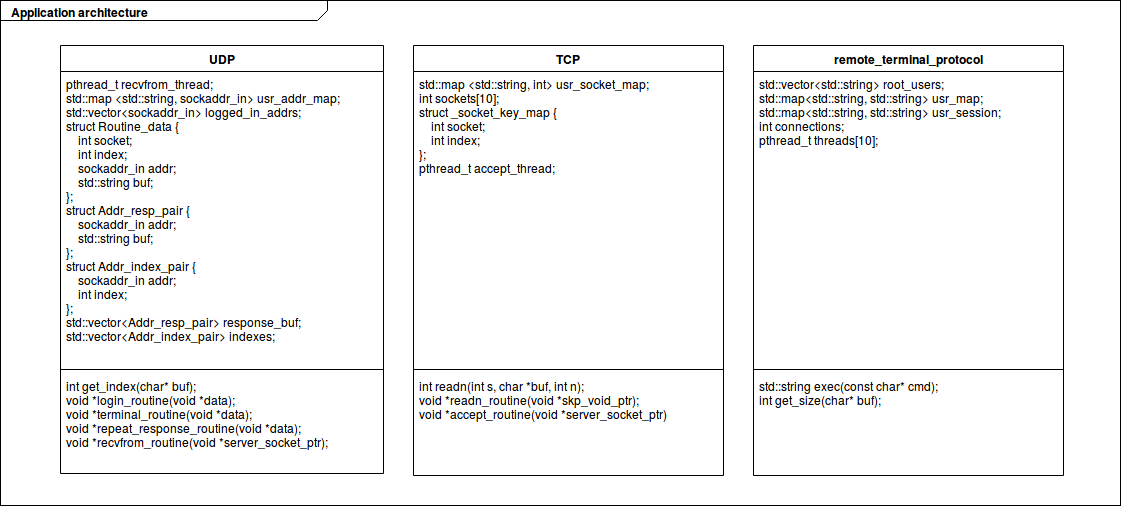
\includegraphics[width=1\textwidth]{pics/arch.png}
\caption{Диаграмма модулей}
\label{diag_mod}
\end{figure}

\subsection{Модуль UDP}
\begin{itemize}
\item[-] recvfrom_thread - дескриптор потока приёма всех входящих запросов
\item[-] usr_addr_map - структура данных, хранящая имя пользователя и соответсвующий данному имени адрес и порт подключения. Необходима для определения адреса отправки ответа по имени пользователя
\item[-] logged_in_addrs - список адресов подключенных пользователей. С помощью него можно определить - входящих пакет поступает от нового подключения или является пакетом сессии одного из уже подклченных пользователей
\item[-] Routine_data - структура данных, содержащая основную информацию для отправки ответа на входящих запрос. Используется для удобной траспортировки данных между потоками
\item[-] Addr_resp_pair - структура данных, объединяющая буфер ответа с адресом пользователя
\item[-] Addr_index_pair - структура данных для хранения данных нумерации пакетов в соответствии с адресом пользователся 
\item[-] response_buf - буфер, хранящий предыдущий ответ для заданного адреса. Данные хранятся парами - каждому адресу ставится в соответствие определенный буфер с ответом. Таким образом можно однозначно получить предыдущий ответ для конкретного адрса, в случае повторного постуления пакета запроса
\item[-] indexes - массив пар адрес:номер пакета. Обеспечивает хранение индексов пакетов индивидуально для каждой сессии
\item[>] get_index - функция распаковки значения индекса принятого запроса
\end{itemize}

\subsection{Модуль TCP}
\begin{itemize}
\item[-] usr_socket_map - структура данных для хранения пар имя_ползователя:дескриптор_сокета. Позволяет соотнести заданного пользователя к конкретному сокету
\item[-] sockets - массив дескрипторов активных сокетов
\item[-] socket_key_map - структура данных для удобного передачи информации между потоками
\item[-] accept_thread - дескриптор потока приёма всех входящих запросов
\end{itemize}


\subsection{Модуль remote_terminal_protocol}
\begin{itemize}
\item[-] root_users - список имён пользователей, обладающих привилигированными правами
\item[-] usr_map - пары логин:пароль зарегистрированные для доступа к удалённому терминалу
\item[-] usr_session - пара имя_пользователя:текущая_директория
\item[-] connections - счётчик активных подключений к серверу. Контролирует входящую нагрузку 
\item[>] exec - функция вызова входящей команды в терминале сервера
\item[>] get_size - функция распаковки значения фактической длины параметров принятого запроса
\end{itemize}

\section{Особенности реализацции}

\subsection{Приложение на основе TCP}

\subsubsection{Серверное приложение}

При запуске серверного приложения, в главном потоке main thread создаётся сокет и устанавливается на прослушку порта 7500. После чего пораждается поток принятия новых соединений accept thread с функцией обработчиком accept_routine(), куда передаётся дескприптор созданного сокета. Accept_routine() в бесконечном цикле принимет новые подключеня, порождая новые потоки readn thread  с назначенной функцией-обработчиком readn_routine(). Readn_routine() в бесконечном цикле принимает входящие данные с помощью функции readn, которая гарантирую целостность принятых данных. Затем, в том же потоке  происходит аутентификация пользователся, отправка дескриптора результата входа в систему и в случае успешного входа в систему - выполнение переданной команды с последующим отправлением результата. По окнчанию соединения, все потоки завершаются. Это гарантируется вызовом функции pthread_join(). Чтобы избежать конфликтов доступа и перезаписи данных, используются мьютексы. Примерное отображение процесса попрождения и завершения потоков отображено на Рис.\ref{tcp_thr}.

\begin{figure}[H]
\centering
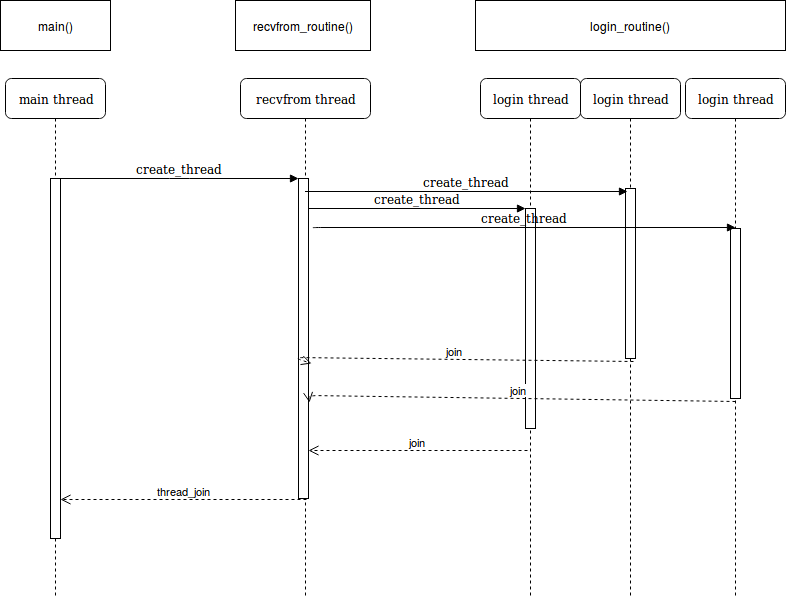
\includegraphics[width=1\textwidth]{pics/tcpthread.png}
\caption{Диаграмма примера потоков в серверном приложении TCP}
\label{tcp_thr}
\end{figure}

\subsubsection{Клиентское приложение}

Клиентское приложение является однопоточным. Создаётся сокет, по которому происходит общение клиента с сервером. Адрес сервера и номер порта для подключения задаются явно. Взаимодействие с сервером происходит последовательно в двух циклах. Первый цикл бесконечный с условием выхода по положительному ответу сервера на запрос доступа к удалённому терминалу. Во втором бесконечном цикле происходит обработка пользовательского ввода с клавиатуры, упаковка передаваемых данных в соответстви с протоколом \ref{tab:request_command} и отправка посредством команды send с последующим принятием ответа через функцию readn(). Выход из второго и цикла и завершение работы клиента происходит либо при вводе пользователем команды logout, либо по решению администратора, либо по принудительной остановке работы сервера.

\subsection{Приложение на основе UDP}
\subsubsection{Серверное приложение}

В приложении с использованием UDP аналогично TCP создаётся сокет, привязываеммый к конкретному порту, в нашем случае к порту 7500. В отличие от TCP никакого принятия новых соединений не происходит. В попрождённом потоке recvfrom thread в функции recvfrom_routine напрямую принимаются UDP дэйтаграммы. Определение необходимого сеанса происходит по адрему отправителя. После принятия дэйтаграммы, определения её принадлежности к одной из активных сессий, а также проверки корректности индекса пакета, происходит попрождение нового потока-обработчика с выполнением соответсвующей запросу функцией: login_routine или terminal_routine. Для ускорения работы сервера, в случае повторного приёма одного и того же пакета, порождается поток с фуекцией обработчик repeat_response_routine() - дублирующей предыдущий ответ по данному запросу. Пример порождения и завершения работы потоков представлен на Рис.\ref{udp_thr}.

\begin{figure}[H]
\centering
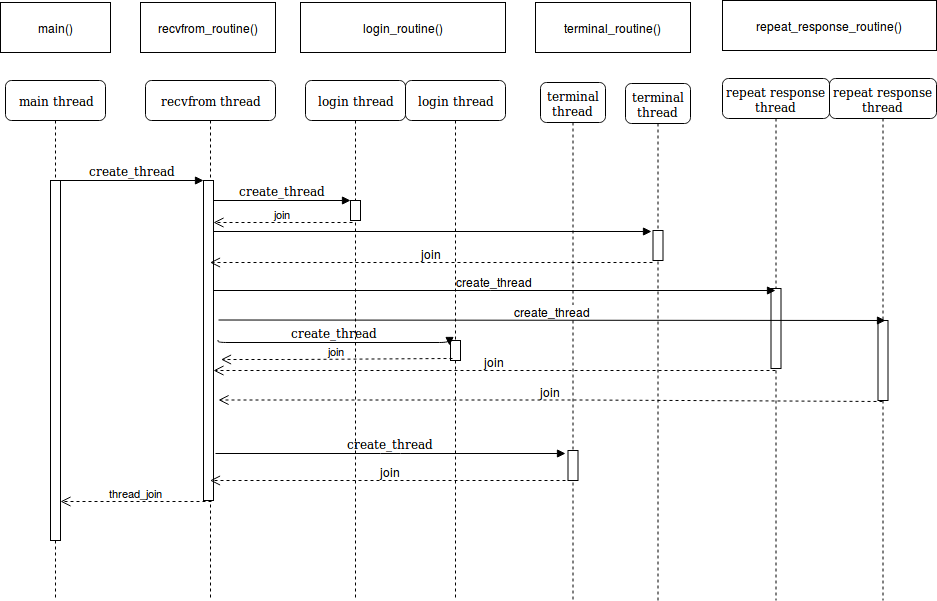
\includegraphics[width=1\textwidth]{pics/udpthread.png}
\caption{Диаграмма примера потоков в серверном приложении UDP}
\label{udp_thr}
\end{figure}
\subsubsection{Клиентское приложение}

\section{Результаты тестирования}

\section{Выводы}



\end{document}
